\subsection{函数}
\paragraph{}
在数集上的映射,$D \subset R$,$f:D \to R$ 称为函数。

\subsection{函数的表示}

\begin{enumerate}
  \item 表格法
  \item 图形法
  \item  解析法(公式法)
\end{enumerate}

\subsection{函数的特性}

\subsubsection{有界性}

\begin{enumerate}
  \item 上界:存在数 $K_1$,满足 $\forall{x},\ f(x) \leq K_1$
  \item 下界:存在数 $K_2$,满足 $\forall{x},\ f(x) \geq K_2$
  \item 有界:存在正数 $M$,满足 $\forall{x},\ |f(x)| \leq M$
  \item 无界:不存在 $M$ 使得第 3 点的公式成立
\end{enumerate}

\subsubsection{单调性}
\paragraph{}
在区间上的单调性:设函数 $f(x)$ 的定义域为 $D$ ,在区间 $I \subset D$ 上的任意两点 $x_1, x_2$,且 $x_1 < x_2$,恒有:

\begin{enumerate}
  \item 单调增加:$f(x_1) < f(x_2)$
  \item 单调减少:$f(x_1) > f(x_2)$
\end{enumerate}

\subsubsection{奇偶性}
\paragraph{}
函数 $f(x)$ 的定义域 $D$ 关于原点对称,如果 $\forall x \in D$,满足:

\begin{enumerate}
  \item 偶函数:$f(-x) = f(x)$
  \item 奇函数:$f(-x) = -f(x)$
\end{enumerate}

\subsubsection{周期性}
\paragraph{}
设函数 $f(x)$ 的定义域为 $D$,存在正整数 $l$,使得任一 $x \in D$,有 $(x \pm l) \in D$,且
 $f(x + l) = f(x)$ 恒成立。

\subsection{反函数与复合函数}

\subsubsection{反函数}
\paragraph{}
设函数 $f:D \rightarrow f(D)$ 是单射,则它存在逆函数 $f^{-1}:f(D) \rightarrow D$,称此函数 $f^{-1}$ 为 $f$ 的反函数。

\subsubsection{复合函数}
\paragraph{}
设函数 $y = f(u)$ 的定义域为 $D_f$,函数 $u = g(x)$ 的定义域为 $D_g$ 且其值域 $R_g \subset D_f$,则由下式确定的函数:

\begin{equation}
y = f[g(x)], x \in D_g
\end{equation}

\paragraph{}
称为由函数 $u = g(x)$ 与函数 $y = f(u)$ 构成的复合函数,变量 $u$ 称为中间变量。

\subsection{函数的运算}
\paragraph{}
设函数 $f(x), g(x)$ 的定义域分别是 $D_1, D_2$,$D = D_1 \cap D_2 \neq \varnothing$,则可以定义下列运算:

\begin{enumerate}
  \item 和(差)$f \pm g$:$(f \pm g)(x) = f(x) \pm g(x), x \in D$
  \item 积$f \cdot g$:$(f \cdot g)(x) = f(x) \cdot g(x), x \in D$
  \item 商$\frac{f}{g}$:$(\frac{f}{g})(x) = \frac{f(x)}{g(x)}, x \in D  \backslash \{x|g(x) = 0, x \in D\}$
\end{enumerate}

\subsection{初等函数}

\begin{enumerate}
  \item 幂函数
  \item 指数函数
  \item 对数函数
  \item 三角函数
  \item 反三角函数
\end{enumerate}

\subsection{双曲函数}
\subsubsection{双曲正弦}
\paragraph{}
$sh \, x = \frac{e^x - e^{-x}}{2}$

\begin{figure}[H]
  \centering
    % sh(x) = (e^x - e^(-x)) / 2
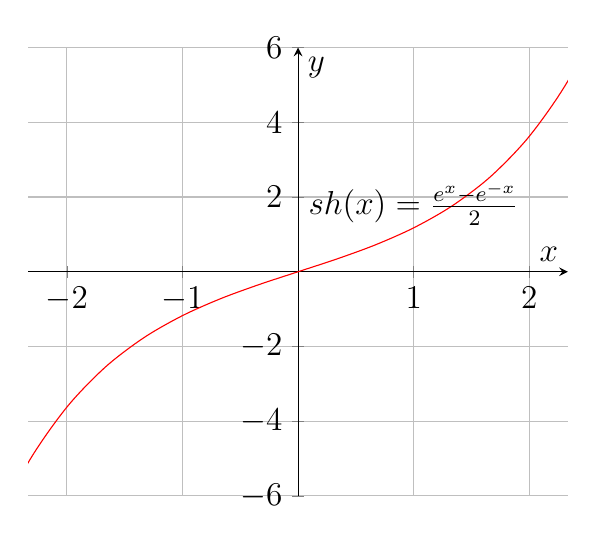
\begin{tikzpicture}
  \begin{axis}[domain=-4:4,ymin=-6,ymax=6, grid=both, font=\large, axis lines = middle, smooth, xlabel={$x$}, ylabel={$y$}]
    \addplot[draw=red] {(e^x - e^(-x)) / 2};
    \node at (axis cs:1,1.8) {$sh(x) = \frac{e^x - e^{-x}}{2}$};
  \end{axis}
\end{tikzpicture}

    \caption{$sh(x) = \frac{e^x - e^{-x}}{2}$}
    \label{sh_x}
\end{figure}

\subsubsection{双曲余弦}
\paragraph{}
$ch \, x = \frac{e^x + e^{-x}}{2}$

\begin{figure}[H]
  \centering
    % ch(x) = (e^x + e^(-x)) / 2
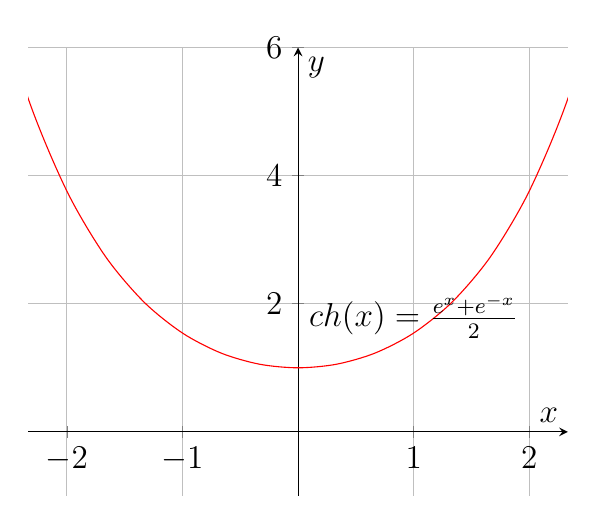
\begin{tikzpicture}
  \begin{axis}[domain=-4:4,ymin=-1,ymax=6, grid=both, font=\large, axis lines = middle, smooth, xlabel={$x$}, ylabel={$y$}]
    \addplot[draw=red] {(e^x + e^(-x)) / 2};
    \node at (axis cs:1,1.8) {$ch(x) = \frac{e^x + e^{-x}}{2}$};
  \end{axis}
\end{tikzpicture}

    \caption{$ch(x) = \frac{e^x + e^{-x}}{2}$}
    \label{ch_x}
\end{figure}

\subsubsection{双曲正切}
\paragraph{}
$th \, x = \frac{sh \, x}{ch \, x} = \frac{e^x - e^{-x}}{e^x + e^{-x}}$


\begin{figure}[H]
  \centering
    % th(x) = (e^x - e^(-x)) / (e^x -+e^(-x))
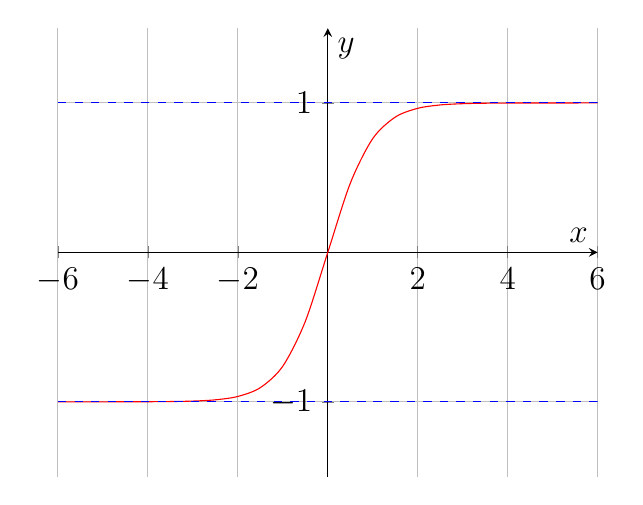
\begin{tikzpicture}
  \begin{axis}[domain=-6:6,ymin=-1.5,ymax=1.5, grid=both, font=\large, axis lines = middle, smooth, xlabel={$x$}, ylabel={$y$}]
    \addplot[draw=red] {(e^x - e^(-x)) / (e^x + e^(-x))};
    \addplot[dashed, draw=blue] {-1};
    \addplot[dashed, draw=blue] {1};
    \node at (axis cs:1,1.8) {$th(x) = \frac{e^x - e^{-x}}{e^x + e^{-x}}$};
  \end{axis}
\end{tikzpicture}

    \caption{$th(x) = \frac{e^x - e^{-x}}{e^x + e^{-x}}$}
    \label{th_x}
\end{figure}

\subsection{反双曲函数}
\subsubsection{反双曲正弦}
\paragraph{}
$y = arsh \, x = \ln(x + \sqrt{x^2 + 1})$

\begin{figure}[H]
  \centering
    % y = arsh(x)
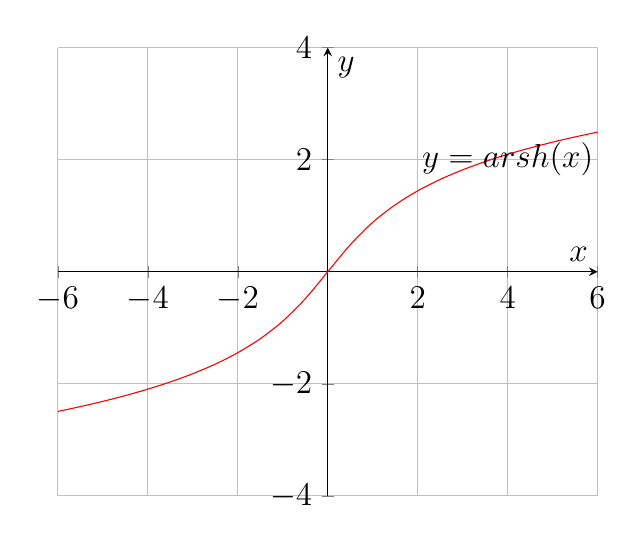
\begin{tikzpicture}
  \begin{axis}[domain=-6:6,ymin=-4,ymax=4, grid=both, font=\large, axis lines = middle, smooth, xlabel={$x$}, ylabel={$y$}]
    \addplot[draw=red] {ln(x + sqrt(x^2 + 1))};
    \node at (axis cs:4,2) {$y = arsh(x)$};
  \end{axis}
\end{tikzpicture}

    \caption{$y = arsh(x)$}
    \label{arsh_x}
\end{figure}

\subsubsection{反双曲余弦}
\paragraph{}
$y = arch \, x = \ln(x + \sqrt{x^2 - 1})$

\begin{figure}[H]
  \centering
    % y = arch(x)
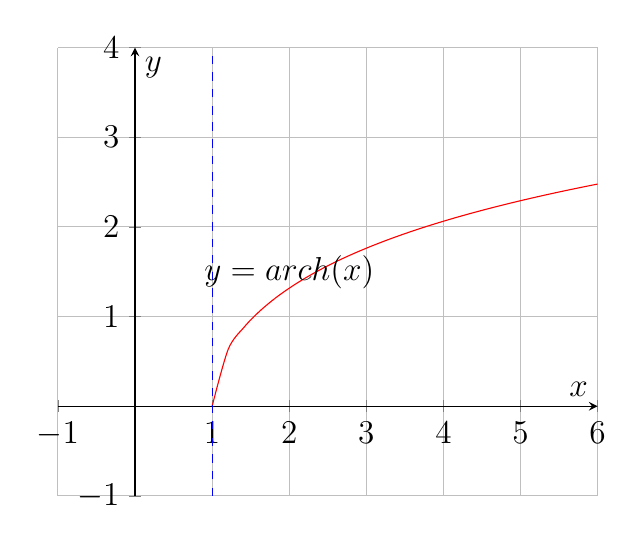
\begin{tikzpicture}
  \begin{axis}[xmin=-1, xmax=6,ymin=-1,ymax=4, grid=both, font=\large, axis lines = middle,
    smooth, xlabel={$x$}, ylabel={$y$}]
    \addplot[draw=red,domain=1:6] {ln(x + sqrt(x^2 - 1))};
    \addplot[dashed, draw=blue, mark=none] coordinates {(1, -1) (1, 4)};
    \node at (axis cs:2,1.5) {$y = arch(x)$};
  \end{axis}
\end{tikzpicture}

    \caption{$y = arch(x)$}
    \label{arch_x}
\end{figure}

\subsubsection{反双曲正切}
\paragraph{}
$y = arth \, x = \frac{1}{2} \ln(\frac{1 + x}{1 - x})$

\begin{figure}[H]
  \centering
    % y = arth(x)
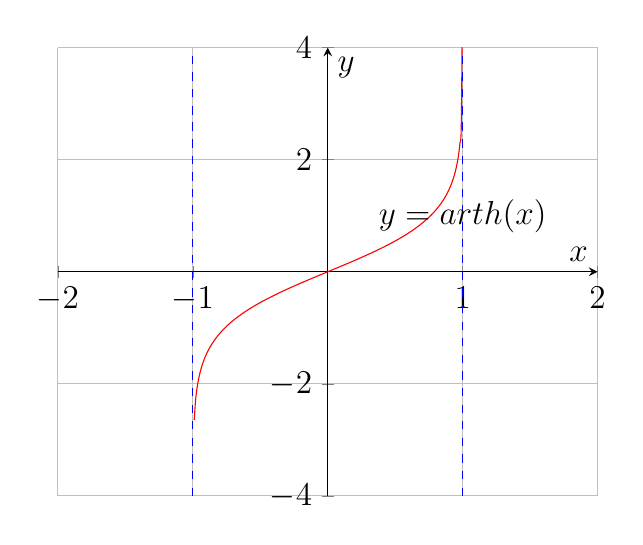
\begin{tikzpicture}
  \begin{axis}[xmin=-2,xmax=2,ymin=-4,ymax=4, grid=both, font=\large, axis lines=middle, smooth, xlabel={$x$}, ylabel={$y$}]
    \addplot[draw=red,domain=-1:1,samples=200] {(1/2)*ln((1 + x)/(1 - x))};
    \addplot[dashed, draw=blue, mark=none] coordinates {(1, -4) (1, 4)};
    \addplot[dashed, draw=blue, mark=none] coordinates {(-1, -4) (-1, 4)};
    \node at (axis cs:1,1) {$y = arth(x)$};
  \end{axis}
\end{tikzpicture}

    \caption{$y = arth(x)$}
    \label{arth_x}
\end{figure}
